\documentclass[11pt]{article}
\usepackage[margin=1in]{geometry}
\usepackage{booktabs,amsmath,amssymb,graphicx,hyperref,xcolor,natbib}
\graphicspath{{./}}
\usepackage{tikz}
\usetikzlibrary{arrows.meta,decorations.pathreplacing,positioning}

\title{Reading Between the Lines:\\Recovering Unrecorded Moves from Chess Scoresheets}
\author{Subhash Bylaiah}
\date{}

\begin{document}
\maketitle

\begin{abstract}
Over-the-board chess games are recorded by hand, and the records are often incomplete: players stop writing in time trouble, skip moves, and make slips. Existing scoresheet tools recognise what was written and flag illegal moves, but leave unwritten moves for the user to type.
We study reconstructing moves that were \emph{never written}, in an interactive setting where a user confirms one move at a time from a short list of suggestions.
We release a benchmark built from public games, with a scoresheet simulator and user-facing metrics.
Our model reads the board and the \emph{rest of the scoresheet}, is trained to predict the board at the next written move, and is combined with a pretrained human-move model (Maia-3). It ranks the true move first 66.4\% of the time and in the top two 82.6\% of the time; a user types 0.66 moves per game, and 61\% of games need no typing. The prior alone ranks the true move first 55.6\% of the time.
On real handwritten scoresheets, real player slips cost about one point. Accuracy is lower on real tournament games, which we trace to slow, classical play; fine-tuning on tournament games recovers about 40\% of this gap, and the final system reaches 75.0\% top-2 on real handwritten sheets.
\end{abstract}

%======================================================================
\section{Introduction}

In over-the-board (OTB) chess, each player writes every move on a paper scoresheet. These records are the only source for publishing, rating disputes and later study, but they are often incomplete. In time trouble, players may legally stop recording, so whole stretches of a game are missing; elsewhere, entries are wrong (``Nd3'' for ``Nb3'') or misread when digitised. Incomplete records hurt most where they matter most for learning: developing players, who are less practised at recording under time pressure, benefit most from reviewing their games, and the unrecorded stretches are often the decisive ones.

Scoresheet digitisation has been studied as handwriting recognition \citep{eicher2021hcs,majid2022digitization,hayashi2022attention}, and recent work repairs \emph{misread} written moves at the level of the whole game \citep{trippen2026zugwise}. These systems depend on something having been written: when the true move is absent from every recognition candidate, the operator types it, which Zugwise reports for at least one move in 43 of its 45 evaluation games. Moves that were never written, often several in a row, remain a manual task.

We address this task directly. Given a scoresheet with known empty boxes and noisy written entries, we rank the legal moves at each unrecorded ply. A user confirms one move at a time: tap one of the top two suggestions, expand to five, or type the move (Figure~\ref{fig:task}).

% Figure: the task. A scoresheet with a time-pressure gap; the assisted loop at one missing ply.
\begin{figure}[t]
\centering
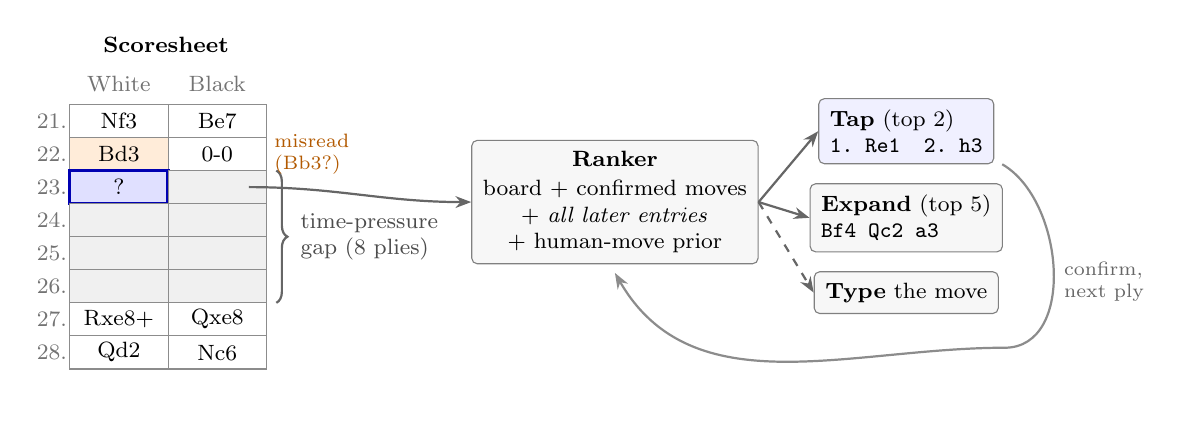
\begin{tikzpicture}[
  font=\footnotesize,
  cell/.style={draw=black!45, minimum width=1.25cm, minimum height=0.42cm, inner sep=1pt},
  num/.style={minimum width=0.55cm, minimum height=0.42cm, text=black!55},
  blank/.style={cell, fill=black!6},
  cur/.style={cell, fill=blue!12, draw=blue!70!black, very thick},
  err/.style={cell, fill=orange!15},
  box/.style={draw=black!50, rounded corners=2pt, inner sep=4pt, align=left},
  arr/.style={-{Stealth[length=2mm]}, thick, black!60},
]
% ---- scoresheet ----
\node[font=\footnotesize\bfseries] at (1.2,0.55) {Scoresheet};
\node[num] at (-0.2,0) {};
\node[text=black!55] at (0.6,0.05) {White}; \node[text=black!55] at (1.85,0.05) {Black};
\def\rows{{"21","22","23","24","25","26","27","28"}}
\foreach \i/\n in {1/21,2/22,3/23,4/24,5/25,6/26,7/27,8/28} {\node[num] at (-0.25,-\i*0.42) {\n.};}
% row 21-22 written
\node[cell] at (0.6,-0.42) {Nf3};   \node[cell] at (1.85,-0.42) {Be7};
\node[err]  at (0.6,-0.84) {Bd3};   \node[cell] at (1.85,-0.84) {0-0};
% gap rows 23-26
\node[cur]  at (0.6,-1.26) {?};     \node[blank] at (1.85,-1.26) {};
\node[blank] at (0.6,-1.68) {};     \node[blank] at (1.85,-1.68) {};
\node[blank] at (0.6,-2.10) {};     \node[blank] at (1.85,-2.10) {};
\node[blank] at (0.6,-2.52) {};     \node[blank] at (1.85,-2.52) {};
% written again 27-28
\node[cell] at (0.6,-2.94) {Rxe8+}; \node[cell] at (1.85,-2.94) {Qxe8};
\node[cell] at (0.6,-3.36) {Qd2};   \node[cell] at (1.85,-3.36) {Nc6};
\draw[decorate, decoration={brace, amplitude=4pt}, thick, black!60] (2.6,-1.05) -- (2.6,-2.73)
  node[midway, right=5pt, align=left, text=black!70] {time-pressure\\gap (8 plies)};
\node[text=orange!70!black, align=left, font=\scriptsize] at (3.05,-0.84) {misread\\(Bb3?)};

% ---- model ----
\node[box, minimum width=2.6cm, align=center, fill=black!3] (model) at (6.9,-1.45)
  {\textbf{Ranker}\\[1pt] board + confirmed moves\\ + \emph{all later entries}\\ + human-move prior};
\draw[arr] (2.25,-1.26) to[out=0,in=180] (model.west);

% ---- suggestions ----
\node[box, fill=blue!6, minimum width=2.2cm] (top2) at (10.6,-0.55) {\textbf{Tap} (top 2)\\ \texttt{1.\ Re1}\quad \texttt{2.\ h3}};
\node[box, fill=black!3, minimum width=2.2cm] (top5) at (10.6,-1.65) {\textbf{Expand} (top 5)\\ \texttt{Bf4 Qc2 a3}};
\node[box, fill=black!3, minimum width=2.2cm] (type) at (10.6,-2.6) {\textbf{Type} the move};
\draw[arr] (model.east) -- (top2.west);
\draw[arr] (model.east) -- (top5.west);
\draw[arr, dashed] (model.east) -- (type.west);
\draw[arr, black!45] (top2.south east) ++(0.1,0) to[out=-30,in=0] node[pos=0.55, right, font=\scriptsize, text=black!60, align=left] {confirm,\\next ply} (11.85,-3.3) to[out=180,in=-60] (6.9,-2.35);
\end{tikzpicture}
\caption{The assisted reconstruction task. Moves 23--26 were not recorded (time pressure), and a written entry may be misread. At each missing ply, the system ranks the legal moves using the confirmed moves, everything written later on the sheet, and a human-move prior. The user taps one of the top two, expands to five, or types the move; the game then advances to the next missing ply. We measure top-$k$ accuracy and how often the user must type.}
\label{fig:task}
\end{figure}


\paragraph{Contributions.}
\begin{enumerate}
  \item \textbf{Task and benchmark.} Gap-aware game reconstruction in a user-assisted setting, with a public benchmark, a scoresheet simulator, and metrics of user effort.
  \item \textbf{A model that reads the rest of the sheet.} A transformer over the board and up to 48 later written entries, with exact ply offsets, trained with an auxiliary task of predicting the board at the next written moves. This task accounts for almost all of the gain from reading ahead.
  \item \textbf{Combining with a pretrained human-move prior.} Adding Maia-3's \citep{maia3} scores and fusing it through gated cross-attention adds about 8 points of top-1 and top-2 accuracy. Most of this comes from the prior itself; the cross-attention adds about one point.
  \item \textbf{Analysis and real data.} Model size, data and move history do not limit accuracy; move order and slow play do. We evaluate on real handwritten scoresheets and real tournament games.
\end{enumerate}

%======================================================================
\section{Related work}

\paragraph{Scoresheet recognition.}
\citet{eicher2021hcs} introduced the Handwritten Chess Scoresheet (HCS) dataset (158 games, 215 page images) and a CNN-BiLSTM recogniser; \citet{majid2022digitization} added legality checks and a semi-automatic mode, and \citet{hayashi2022attention} study attention-based recognisers. Commercial apps convert photos to PGN and flag illegal moves. All leave missing moves to the user.

\paragraph{Game-level repair.}
Zugwise \citep{trippen2026zugwise} aligns both players' sheets and ranks replacements for misread moves using recogniser confidence and a Maia-style prior. Its ranking evaluation covers 45 real club games, on decisions where the correct move is among the recogniser's candidates; moves written on neither sheet must be typed by the operator. These unwritten moves are our task. Enumerating legal fillings of a gap \citep{narayanan2019missing} keeps every consistent continuation, but does not rank them and grows exponentially with gap length.

\paragraph{Human move prediction and chess transformers.}
Maia \citep{maia1}, Maia-2 \citep{maia2}, Allie \citep{allie} and Maia-3 \citep{maia3} predict human moves from the position, with skill conditioning; Maia-3 reaches 55--57\% top-1 on Lichess blitz. Square-token transformers with a from--to move head \citep{monroe2024mastering,maia3} are the basis of our board encoding. RePAIR \citep{repair} predicts masked positions in a learned representation space, for representation learning rather than move recovery.

%======================================================================
\section{Task and benchmark}
\label{sec:task}

\paragraph{Assisted reconstruction.} A scoresheet has one box per ply, written or empty. Empty boxes are visible, so the positions and lengths of the gaps are known. At each unrecorded ply, given the confirmed moves so far, the system ranks the legal moves; the user confirms the true move and the game advances (formalised in \S\ref{sec:formulation}).

\paragraph{Metrics.} Top-$k$ accuracy over missing plies ($k=1,2,5$), matching a three-tier interface: \emph{tap} if the true move is in the top 2, \emph{expand} if in the top 5, otherwise \emph{type}. We also report typed moves per game and the share of games needing no typing.

\paragraph{Simulator.} We damage complete games and keep full ground truth. The main process is a \emph{time-pressure burst}: one run of 4--40 consecutive unrecorded plies, placed preferentially late in the game. Further processes add isolated forgotten moves, OCR-style misreadings (confusable characters, with optional n-best alternatives), player \emph{slips} (a wrong move written cleanly), stray entries, and formatting variation. Presets combine them; we report on the three with gaps: \texttt{missing} (a burst only), \texttt{mixed} (a burst and light errors) and \texttt{mixed\_ocr} (heavier misreadings with n-best lists). Rates are in Appendix~\ref{app:sim}.

\paragraph{Data.} Lichess rated games \citep{lichessdb} (CC0) from 2026, split by game-id hash; the training sets hold 500k and 2M games (72\% blitz, 27\% rapid, 1\% classical). The \textbf{test} set has 200 September-2026 games (507 instances with gaps, 5,871 missing plies); a \textbf{dev} set of 200 further held-out games (5,787 missing plies) is used for every tuning decision. Maia-3 was trained on games up to July 2025.

\paragraph{Unknown layout (not studied).} If gap positions are unknown (e.g.\ only a list of written moves survives), one must also infer which ply each entry records, an \emph{alignment}, and reconstruct the game automatically. An early version of our system recovered whole games exactly for 28.7\% of sheets with gaps of 1--4 plies and for none with 10 or more. Since about a quarter of missing plies are ambiguous even given the rest of the sheet (\S\ref{sec:errors}), we study the assisted setting. Our final model relies on known gap positions and was not evaluated here.

%======================================================================
\section{Method}
\label{sec:method}

The system has four parts (Figure~\ref{fig:arch}): a scoresheet tower that scores moves from the board and the written record, a pretrained human-move tower fused into it, a feasibility filter, and a short evidence search near written moves.

% Figure: architecture. Scoresheet tower (left), gated cross-attention (middle), Maia-3 tower (right), then combination, filter + search.
\begin{figure*}[t]
\centering
\resizebox{\textwidth}{!}{%
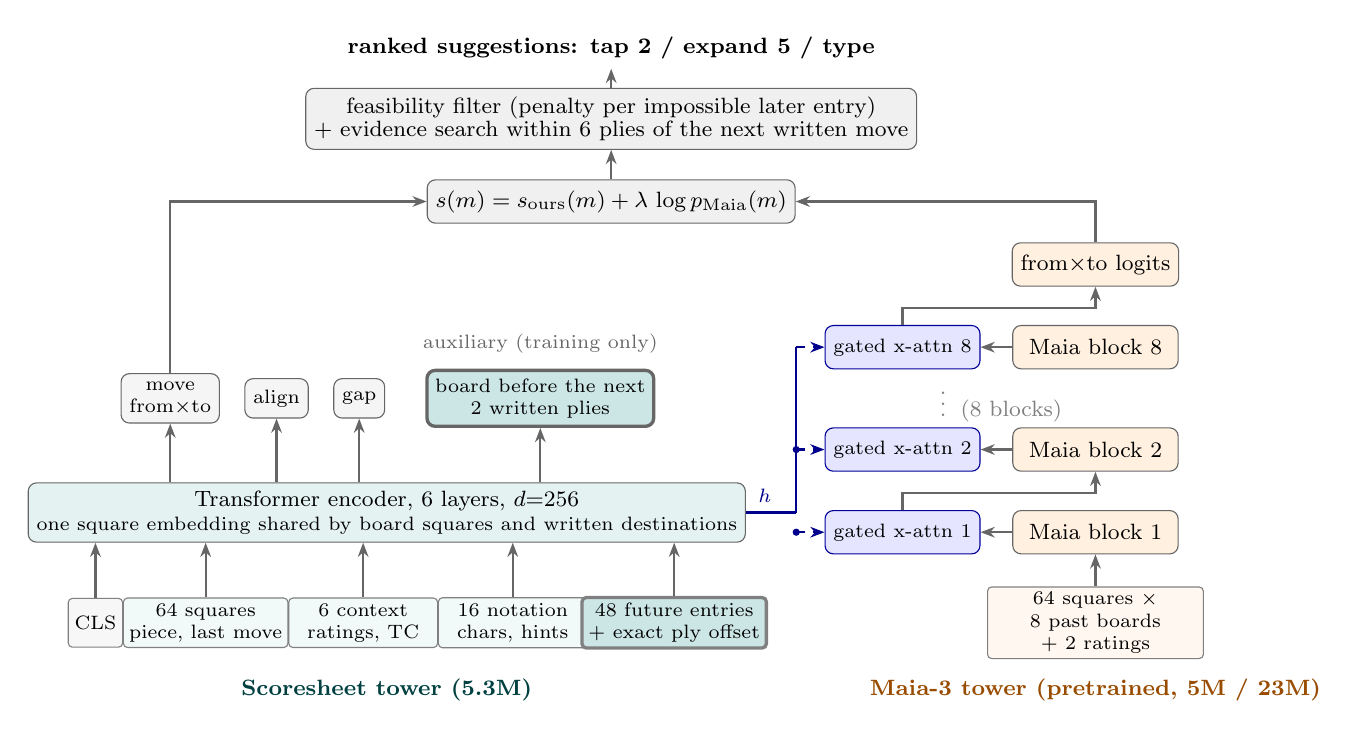
\begin{tikzpicture}[
  font=\footnotesize,
  tok/.style={draw=black!50, rounded corners=1.5pt, minimum height=0.62cm, inner sep=2pt, align=center, font=\scriptsize},
  blk/.style={draw=black!60, rounded corners=3pt, minimum height=0.55cm, inner sep=3pt, align=center},
  ours/.style={blk, fill=teal!10},
  maia/.style={blk, fill=orange!12},
  fuse/.style={blk, fill=blue!10, draw=blue!60!black, font=\scriptsize},
  head/.style={blk, fill=black!4, minimum height=0.5cm, font=\scriptsize},
  arr/.style={-{Stealth[length=1.8mm]}, thick, black!60},
  mem/.style={-{Stealth[length=1.8mm]}, thick, blue!55!black, dashed},
  lbl/.style={font=\scriptsize, text=black!60},
]
% ===== scoresheet tower (x 0..7) =====
\node[tok, fill=black!3, text width=0.55cm] (cls) at (-0.55,0) {CLS};
\node[tok, fill=teal!5, text width=1.95cm] (sq) at (0.85,0) {64 squares\\piece, last move};
\node[tok, fill=teal!5, text width=1.75cm] (ctx) at (2.85,0) {6 context\\ratings, TC};
\node[tok, fill=teal!5, text width=1.75cm] (nt) at (4.75,0) {16 notation\\chars, hints};
\node[tok, fill=teal!20, text width=2.2cm, very thick] (fut) at (6.8,0) {48 future entries\\+ exact ply offset};
\node[ours, minimum width=8.9cm] (enc) at (3.15,1.4) {Transformer encoder, 6 layers, $d{=}256$\\[-1pt]{\scriptsize one square embedding shared by board squares and written destinations}};
\foreach \n in {cls,sq,ctx,nt,fut} \draw[arr] (\n.north) -- (\n.north |- enc.south);
\node[head] (hmove) at (0.4,2.85) {move\\from$\times$to};
\node[head] (halign) at (1.75,2.85) {align};
\node[head] (hgap) at (2.8,2.85) {gap};
\node[head, fill=teal!20, very thick] (hfb) at (5.1,2.85) {board before the next\\2 written plies};
\foreach \n in {hmove,halign,hgap,hfb} \draw[arr] (\n.south |- enc.north) -- (\n.south);
\node[lbl] at (5.1,3.55) {auxiliary (training only)};
\node[font=\footnotesize\bfseries, text=teal!50!black] at (3.15,-0.85) {Scoresheet tower (5.3M)};

% ===== gated cross-attention (x ~9) and Maia tower (x ~11.6) =====
\node[tok, fill=orange!6, text width=2.6cm] (mtok) at (12.15,0) {64 squares $\times$\\8 past boards + 2 ratings};
\node[maia, minimum width=2.1cm] (b1) at (12.15,1.15) {Maia block 1};
\node[fuse, minimum width=1.7cm] (f1) at (9.7,1.15) {gated x-attn 1};
\node[maia, minimum width=2.1cm] (b2) at (12.15,2.2) {Maia block 2};
\node[fuse, minimum width=1.7cm] (f2) at (9.7,2.2) {gated x-attn 2};
\node[text=black!50] at (10.95,2.85) {$\vdots$ \;(8 blocks)};
\node[maia, minimum width=2.1cm] (b8) at (12.15,3.5) {Maia block 8};
\node[fuse, minimum width=1.7cm] (f8) at (9.7,3.5) {gated x-attn 8};
\node[maia, minimum width=2.1cm] (mhead) at (12.15,4.55) {from$\times$to logits};
\draw[arr] (mtok.north) -- (b1.south);
\draw[arr] (b1.west) -- (f1.east); \draw[arr] (f1.north) -- ++(0,0.22) -| (b2.south);
\draw[arr] (b2.west) -- (f2.east);
\draw[arr] (b8.west) -- (f8.east); \draw[arr] (f8.north) -- ++(0,0.22) -| (mhead.south);
\node[font=\footnotesize\bfseries, text=orange!60!black] at (12.15,-0.85) {Maia-3 tower (pretrained, 5M / 23M)};
% memory: final scoresheet states h feed every fusion block (a vertical bus)
\coordinate (bus) at (8.35,1.4);
\draw[thick, blue!55!black] (enc.east) -- (bus);
\node[lbl, text=blue!55!black, above] at (7.95,1.4) {$h$};
\draw[thick, blue!55!black] (bus) -- (bus |- f8.west);
\draw[mem] (bus |- f1.west) -- (f1.west);
\draw[mem] (bus |- f2.west) -- (f2.west);
\draw[mem] (bus |- f8.west) -- (f8.west);
\fill[blue!55!black] (bus |- f1.west) circle (1.3pt) (bus |- f2.west) circle (1.3pt);

% ===== combination, filter, search =====
\node[blk, fill=black!6] (comb) at (6.0,5.35) {$s(m)=s_{\text{ours}}(m)+\lambda\,\log p_{\text{Maia}}(m)$};
\draw[arr] (hmove.north) |- (comb.west);
\draw[arr] (mhead.north) |- (comb.east);
\node[blk, fill=black!6, align=center] (post) at (6.0,6.4) {feasibility filter (penalty per impossible later entry)\\[-1pt]+ evidence search within 6 plies of the next written move};
\draw[arr] (comb.north) -- (post.south);
\node[font=\footnotesize\bfseries] (out) at (6.0,7.3) {ranked suggestions: tap 2 / expand 5 / type};
\draw[arr] (post.north) -- (out.south);
\end{tikzpicture}%
}
\caption{Architecture. \textbf{Left:} the scoresheet tower reads the board, context, the nearby notation and up to 48 later written entries, each with its exact ply offset. Its auxiliary head predicts the board before the next two written plies (training only). \textbf{Right:} the pretrained Maia-3 tower reads the last 8 positions and both ratings. After each of its 8 blocks, a gated cross-attention lets the 64 square states read the scoresheet tower's final states $h$; the gates are closed at initialisation, so training starts from Maia-3 exactly. \textbf{Top:} move scores add the two heads with a learned weight $\lambda$, followed by the feasibility filter and the evidence search.}
\label{fig:arch}
\end{figure*}


\subsection{Problem formulation}
\label{sec:formulation}
A game is a sequence of plies $m_1,\dots,m_T$. Its scoresheet has one box per ply, either \emph{written}, holding a string such as ``Nf3'' (optionally with a recogniser's alternative readings), or \emph{empty}. Let $W\subseteq\{1,\dots,T\}$ be the written plies and $w_p$ the text at ply $p\in W$. $W$ is known, but the text may be wrong: the player may have \emph{slipped}, writing a different move, or a correct entry may have been \emph{misread} when digitised.
At a missing ply $i\notin W$, all earlier plies are known (written or confirmed by the user), so they fix the board $b_i$. The task is to rank the legal moves of $b_i$ by
\[
P\big(m_i=m \;\big|\; b_i,\; m_{<i},\; \{w_p\}_{p\in W},\; \text{ctx}\big),
\]
where ctx holds the ratings and time control. The conditioning includes the entries \emph{after} the gap, which constrain how the game continued. Evaluation always continues from the true move, as in an interactive tool where every move is confirmed.

\subsection{Scoresheet tower}
\label{sec:tower}
Inputs are expressed from the side to move (the board and the rank digits of written text are mirrored when Black moves). A 6-layer transformer \citep{vaswani2017attention} ($d=256$, 5.3M parameters) reads 135 tokens:
\begin{itemize}
  \item \textbf{64 square tokens} \citep{monroe2024mastering,maia3}: piece, last-move flag and a learned square embedding. The square embedding is shared with every written mention of that square, so ``destination f3'' in an entry and the f3 token share an identity.
  \item \textbf{Context tokens:} castling, en passant, both ratings and the time control.
  \item \textbf{16 notation tokens:} the next written entries, as text in order. Each entry is encoded from its characters, so misspelled or misread entries keep partial information.
  \item \textbf{48 future tokens:} every later written entry with its parsed move (piece, destination, capture, promotion) and its \emph{exact} ply offset, possible because the gap positions are known. They make the notation tokens largely redundant in our setting; we keep the latter for the unknown-layout case.
\end{itemize}
\textbf{Heads.} The \emph{move} head scores each from--to pair by the scaled dot product of projections of the two square states, as in \citet{monroe2024mastering} and \citet{maia3}, with a separate head for the promotion piece. Three auxiliary heads, used only as training signals, predict whether the current ply is recorded by the next notation token, the number of plies to the next written ply, and the \textbf{board before each of the next two written plies} (13 classes per square, all 64 squares). The board head forces the square states to represent how the game proceeds to the next written moves. All heads use cross-entropy:
\[
\mathcal L=\mathcal L_{\text{move}}+\mathcal L_{\text{align}}+0.1\,\mathcal L_{\text{gap}}+0.1\,\mathcal L_{\text{promo}}+0.2\,\mathcal L_{\text{board}},
\]
with weights set by hand. Training samples every unrecorded ply (and a quarter of written plies) from games corrupted on the fly with a mixture of presets, for 100k steps of 256 positions (Appendix~\ref{app:model}).

\subsection{Fusion with a pretrained human-move prior}
\label{sec:fusion}
Maia-3 \citep{maia3} reads 64 square tokens holding the last 8 positions and soft embeddings of both ratings, and produces from--to logits. We use its 5M and 23M checkpoints. Following Flamingo \citep{alayrac2022flamingo}, after every Maia block $\ell$ we let its square states $x$ attend to our tower's final states $h$ through gates initialised at zero:
\begin{align*}
x &\leftarrow x+\tanh(g_a^{(\ell)})\,\mathrm{MHA}\big(Q\!=\!\mathrm{LN}(x),\;K\!=\!V\!=\!W^{(\ell)}\mathrm{LN}(h)\big),\\
x &\leftarrow x+\tanh(g_f^{(\ell)})\,\mathrm{FF}(x).
\end{align*}
MHA has its own learned projections; $W^{(\ell)}$ maps our 256-dimensional states to Maia's width, and FF is a small feed-forward network. At initialisation the Maia tower is exactly the pretrained model. The final move score is
\[
s(m)=s_{\text{ours}}(m)+\lambda\,\log p_{\text{Maia}}(m),
\]
with $\lambda$ learned (initialised at 1.5, the best weight for the untrained sum). We fine-tune for 50k steps, with the pretrained towers at $0.1\times$ the learning rate. The 23M hybrid has 46.1M parameters.

\subsection{Feasibility filter and evidence search}
\label{sec:search}
The \textbf{filter} checks necessary conditions for every later written entry to stay reachable (castling rights, whether the moving piece can reach its written destination in time, whether a written capture has a target), and subtracts a penalty for each violation, since a slip can make the true move look infeasible.
The \textbf{search} applies when the next written ply is at most $D$ plies away: each of the model's top 10 candidates is played forward with a width-8 beam through the gap and the next written plies, scoring how well each path matches the written entries under a noisy observation model; a candidate's score is its prior plus the log-sum-exp of its paths. Beyond $D$ plies we rank by the model alone. $D=6$ and the penalty were chosen on the dev set (Appendix~\ref{app:search}).

%======================================================================
\section{Results}

\begin{table}[t]
\centering
\small
\begin{tabular}{lccccc}
\toprule
Method & Top-1 & Top-2 & Top-5 & Typed/game & No typing \\
\midrule
Chance & 6.9 & 12.4 & 24.1 & -- & -- \\
Legality + feasibility only & 9.6 & 15.8 & 27.7 & -- & -- \\
Early tower (no future entries), model only & 41.1 & -- & 76.6 & 2.71 & -- \\
\quad + filter + search & 46.7 & 61.2 & 78.9 & 2.44 & 27\% \\
\quad trained $3.3\times$ longer, + filter + search & 57.4 & 74.1 & 89.2 & 1.25 & 45\% \\
Scoresheet tower (\S\ref{sec:tower}) + filter + search & 58.4 & 75.0 & 89.8 & 1.18 & 46\% \\
Maia-3 23M alone (no scoresheet) & 55.6 & 74.9 & 91.3 & -- & -- \\
Tower + $1.5\times$ Maia-3 5M, untrained sum, + filter & 62.1 & 78.4 & 92.8 & 0.84 & 54\% \\
Hybrid, Maia-3 5M, model only & 63.4 & 79.9 & 93.4 & 0.76 & 57\% \\
Hybrid, Maia-3 23M, model only & 64.4 & 80.9 & 93.6 & 0.74 & 58\% \\
\textbf{Hybrid 23M + filter + search$^\dagger$} & \textbf{66.4} & \textbf{82.6} & \textbf{94.3} & \textbf{0.66} & \textbf{61\%} \\
\bottomrule
\end{tabular}
\caption{Assisted reconstruction on the test set (5,871 missing plies). Top-$k$ in \%. ``Model only'': no filter and no search (the filter changes the hybrids by $\le$0.1). Search settings were chosen on the dev set; -- means not measured. $^\dagger$The final, OTB-fine-tuned model (\S\ref{sec:otb}) scores identically. 95\% intervals (bootstrap over games): final top-1 [64.7, 68.1], top-2 [81.2, 84.0]; scoresheet tower top-1 [56.7, 60.0], top-2 [73.4, 76.5].}
\label{tab:main}
\end{table}

\paragraph{Main result (Table~\ref{tab:main}).} Rules alone barely beat chance: the filter keeps the true move 98.8\% of the time but leaves a median of 31 candidates. The final system ranks the true move first 66.4\% of the time and in the top two 82.6\%; a user types 0.66 moves per game, and 61\% of games need no typing. Its gain over the scoresheet tower alone is +8.0 top-1 [+6.8, +9.2] and +7.6 top-2 [+6.4, +8.8] (game-clustered 95\% intervals).
Most of this gain comes from the prior: adding the two models' scores without training already raises top-1 from 58.4 to 62.1 (62.7 with Maia-3 23M). Fine-tuning, the larger prior and search add the rest. The cross-attention itself is worth about one point: zeroing all gates at test time lowers validation top-1 from 66.4 to 65.2. Even so, the hybrid beats Maia-3 alone by 10.8 top-1, so the scoresheet evidence matters next to a strong prior.

\begin{figure}[t]
\centering
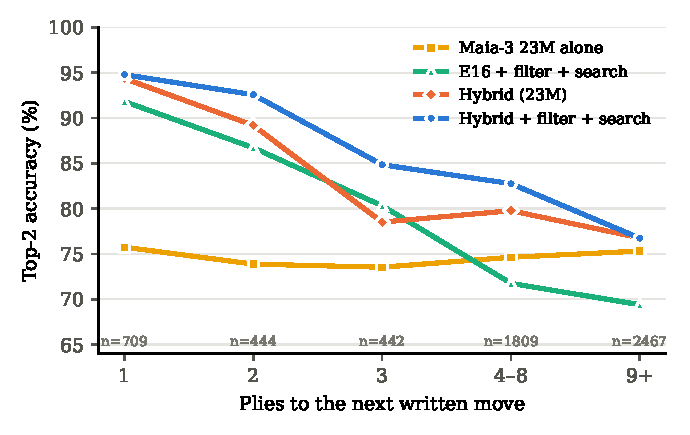
\includegraphics[width=0.62\linewidth]{figs/by_distance.pdf}
\caption{Top-2 accuracy by distance to the next written move (test set). The scoresheet-blind prior is flat; reading the sheet helps most near written moves, and search most at 2--8 plies.}
\label{fig:dist}
\end{figure}

\paragraph{Distance to the next written move} matters most (Figure~\ref{fig:dist}). Top-1 / top-2 fall from 87.3 / 94.8 one ply before a written move to 59.1 / 76.7 at nine or more plies, where all systems approach the prior.

\subsection{Ablations}
\label{sec:ablations}
On the test set, with filter and search unless stated:
\begin{itemize}
  \item \textbf{The board task makes reading ahead work:} without it, top-1 is 55.9 instead of 58.4, about the same as having no future entries. Using 48 rather than 16 future entries adds about 1 point.
  \item \textbf{Capacity and data do not help:} a 15M-parameter tower scores 58.5, and the same tower on 4$\times$ the games 57.6 (5.3M tower: 58.4).
  \item \textbf{Move history does not help:} tokens for the last 8 moves hurt the early tower (41.1 $\to$ 36.4) and change nothing in the hybrid (64.3 vs 64.4), whose Maia tower already reads 8 past boards.
  \item \textbf{Characters versus whole entries:} encoding each written entry as a single token instead of by its characters makes no clear difference (57.4 vs 56.9 top-1, model + filter); characters are slightly ahead next to wrong entries, but not significantly.
  \item \textbf{A larger prior helps a little:} Maia-3 23M rather than 5M adds 1.0 top-1 and top-2.
  \item \textbf{Search adds about 2 points} to the hybrid, mostly 4--8 plies before a written move.
\end{itemize}

\subsection{Error analysis}
\label{sec:errors}
We classify each top-1 miss of the hybrid (model + filter) as an \emph{order} error (the suggested move is played later in the same gap by the same side), an \emph{equivalent} move (the rest of the sheet cannot distinguish it from the true move), or \emph{other}. Order errors are the largest identifiable class: 9.2\% of plies and 39\% of top-2 misses, rising from 0\% one or two plies before a written move to 13.4\% at nine or more. Equivalent moves are 3.3\% and other errors 23.2\%. Even with the true continuation known, 25.5\% of missing plies admit several sheet-consistent moves; only knowledge of how people play can choose among them, which is the prior's role. For the scoresheet tower alone, counting a suggestion as correct when it is played anywhere in the gap raises top-2 to about 85\%: the model largely knows \emph{which} moves were played and loses accuracy on \emph{when}.

%======================================================================
\section{Real data}

\subsection{Real handwritten scoresheets}
HCS \citep{eicher2021hcs} labels each move box with what the player \emph{wrote}, slips included; only 10 of its 207 labelled pages replay legally as written. We recover each page's most likely true game by a search over legal games that minimises edit distance to the written entries, keep 80 games whose recovery is reliable, insert gaps with our \texttt{missing} preset, and keep the \emph{real} written text elsewhere (Appendix~\ref{app:hcs}). In these sheets 5.6\% of visible entries are real slips, within our simulator's range (4.6--9.5\% wrong entries across presets). Common confusions are c$\leftrightarrow$e, f$\leftrightarrow$g, 3/4/5 and R$\leftrightarrow$K/B/Q.

\begin{table}[t]
\centering
\small
\begin{tabular}{lccc}
\toprule
HCS: 80 games, 1,262 missing plies & Top-1 & Top-2 & Top-5 \\
\midrule
Scoresheet tower alone, real written text & 47.7 & 63.5 & 81.5 \\
Hybrid 23M, corrected text & 56.5 & 72.0 & 87.7 \\
Hybrid 23M, real written text & 55.5 & 71.6 & 87.4 \\
Hybrid 23M + OTB fine-tune & 56.8 & 74.2 & 88.2 \\
\textbf{+ filter + search (final system)} & \textbf{58.8} & \textbf{75.0} & \textbf{88.2} \\
\bottomrule
\end{tabular}
\caption{Real scoresheets with simulated gaps (filter, no search unless stated). Final system 95\% intervals: top-1 [55.6, 62.0], top-2 [71.5, 78.2].}
\label{tab:hcs}
\end{table}

Real slips cost about one point (Table~\ref{tab:hcs}), and the hybrid's gain over the scoresheet tower holds (+8). Accuracy is about 9 points below the simulated test set, at every gap size.

\subsection{Real tournament games: the cost of slow play}
\label{sec:otb}
To separate sheet noise from the games themselves, we apply our simulator to real OTB tournament games from the Lichess broadcast database \citep{lichessdb} (September 2026, CC BY-SA 4.0), 150 games per speed (Table~\ref{tab:otb}).

\begin{table}[t]
\centering
\small
\begin{tabular}{lccc}
\toprule
Top-1 / top-2 & OTB blitz & OTB rapid & OTB classical \\
\midrule
Scoresheet tower alone & 54.3 / 71.6 & 53.2 / 70.4 & 48.7 / 64.4 \\
Hybrid 23M & 65.1 / 81.2 & 64.0 / 80.8 & 58.6 / 75.2 \\
Hybrid + OTB fine-tune & 65.6 / 81.7 & 65.6 / 81.9 & 61.5 / 77.8 \\
\textbf{+ filter + search (final system)} & \textbf{67.6 / 83.1} & \textbf{67.2 / 83.2} & \textbf{62.8 / 79.1} \\
\bottomrule
\end{tabular}
\caption{Simulated sheets on real OTB games (filter, no search unless stated). Lichess test set for reference: 64.4 / 80.9, and 66.4 / 82.6 with search.}
\label{tab:otb}
\end{table}

OTB blitz and rapid match online games, so OTB play by itself is not the issue; classical games cost about 6 points. Our training data and Maia-3's are almost entirely fast online games. HCS does not record time controls, but if its games are mostly classical, as is typical for recorded games, this shift would account for most of its drop.

\paragraph{Fine-tuning on OTB games.} We fine-tune the hybrid for 20k steps on 1.08M broadcast games (January 2020 to August 2026, with all games of the evaluation month removed) mixed with 400k Lichess games. Classical accuracy rises by 2.9 top-1 and 2.6 top-2, closing about 40\% of the gap to blitz. On real HCS sheets, top-2 rises by 2.5 [+1.0, +4.1] (top-1 by 1.3 [$-0.3$, +3.1], not yet significant on 80 games). The Lichess test set is unchanged (66.4 / 82.6 / 94.3 with search), so this is our final system.

%======================================================================
\section{Limitations}
Gaps are simulated, also on real sheets, and real gap placement may differ. The HCS truth is recovered automatically, and only 80 of 157 games are kept. We assume an off-the-shelf handwriting recogniser and model its errors rather than evaluating from photographs. Maia expects Lichess ratings, whereas OTB players have FIDE or national ratings. Search costs about 0.6\,s per suggestion on a laptop GPU; searching only within 3 plies is faster and loses about 1 point of top-2. The hybrid builds on Maia-3 (AGPL-3.0), and broadcast data is CC BY-SA.

\section{Release}
Code is released under AGPL-3.0. We release the test and dev benchmarks (CC0), the OTB broadcast benchmark (CC BY-SA 4.0), scripts that rebuild the HCS-derived set from the original HCS release (not redistributed), the simulator and evaluation code with one command per table, and the models: the scoresheet tower (MIT) and the hybrid checkpoints (AGPL-3.0, following Maia-3). Code, data and links to the model checkpoints: \url{https://github.com/subhashbylaiah/chess-game-reconstruction}.

\section{Conclusion}
The unrecorded stretches of a scoresheet are where digitisation tools stop. Treating the rest of the sheet as evidence, and learning to anticipate the board at the next written move, turns them into a ranking task: combined with a human-move prior, a user taps one of two suggestions for 83\% of missing moves, and most games need no typing. The main remaining errors are move order within long gaps and the shift to slow OTB play. Ranking a gap's moves jointly, automatic reconstruction with unknown gap positions, and evaluation from photographs are natural next steps.

\section*{Acknowledgements}
This work was motivated by scoresheets from tournaments run by Chess Cardinals, a non-profit chess club; the author thanks its players and volunteers. AI tools assisted with implementation, experiments and writing; the author is responsible for the work and verified all results.

\bibliographystyle{plainnat}
\bibliography{refs}

%======================================================================
\appendix
\section{Simulator details}
\label{app:sim}
From a complete game (truncated to 80 plies), the simulator produces one or two scoresheets with the true moves, the entry--ply alignment, and the kind of every entry (match, misread, slip, inserted).
\begin{itemize}
  \item \textbf{Time-pressure burst:} one run of unrecorded plies whose length is drawn uniformly from 4 to 40. Its start is drawn with probability proportional to $(s+1)^2$ for a start at ply $s$, so bursts tend to be late. At least two written plies follow it.
  \item \textbf{Isolated drops:} each ply is independently left blank with a small probability.
  \item \textbf{OCR confusion:} 1--2 edits from a table of visually confusable characters (e.g.\ c$\to$e, b$\to$d/h/6, 3$\to$8, 1$\to$7, N$\leftrightarrow$K, B$\to$8/R, Q$\to$O), or a dropped stroke. With n-best output, the written text is the top reading, with a confidence drawn uniformly between 0.45 and 0.95, and the true text is included with probability 0.6.
  \item \textbf{Player slip:} a legal but wrong move with the same destination, or the same piece moving within two squares of the true destination.
  \item \textbf{Inserted entries:} spurious extra entries.
  \item \textbf{Formatting:} move-number hints on 80\% of sheets; check marks stripped and castling written ``0-0'' 30\% of the time each; after a gap, the writer continues in the next row half of the time, shifting the numbering.
\end{itemize}
\begin{table}[h]
\centering\small
\begin{tabular}{lcccccc}
\toprule
Preset & Burst & Drop & OCR & Slip & Insert & n-best \\
\midrule
\texttt{missing} & 1.0 & 0.01 & -- & -- & -- & no \\
\texttt{mixed} & 0.6 & 0.01 & 0.03 & 0.01 & 0.005 & no \\
\texttt{mixed\_ocr} & 0.6 & 0.01 & 0.08 & 0.01 & 0.005 & yes \\
\texttt{substitution} & -- & -- & 0.06 & 0.02 & 0.005 & no \\
\bottomrule
\end{tabular}
\caption{Simulator presets: per-game burst probability; per-ply or per-entry rates otherwise. Written entries that differ from the true move: 4.6\% (\texttt{mixed}), 8.4\% (\texttt{substitution}), 9.5\% (\texttt{mixed\_ocr}). \texttt{clean} and \texttt{two\_sheets} are also released.}
\label{tab:presets}
\end{table}

\section{Model and training details}
\label{app:model}
\paragraph{Tokens.} The input is $1+64+6+16+48=135$ tokens of width 256: content embeddings plus position and token-type embeddings.
\begin{itemize}
  \item Square tokens: piece (13 classes), last-move flag (none / from / to), and square embedding.
  \item Context tokens: castling rights (16), en-passant file (9), each player's rating (26 buckets of 100 points, plus unknown), time-control base (14 buckets) and increment (10 buckets).
  \item Notation tokens: up to 8 characters from a 32-symbol vocabulary; character and character-position embeddings are summed and passed through a two-layer MLP, plus embeddings of the move-number hint (relative offset $-8..{+}24$), recogniser confidence decile, and slot.
  \item Future tokens: the same character encoding, plus parsed fields (piece including castling or unparsed, destination via the shared square embedding, capture, disambiguation file and rank, promotion), the ply offset (exact for 1--16, then buckets up to $>64$), and recogniser confidence.
\end{itemize}
\paragraph{Encoder and heads.} 6 pre-norm layers, 8 heads, feed-forward 1024, GELU, no dropout. Move score $s_{\text{ours}}(f\!\to\!t)=\langle W_q h_f, W_k h_t\rangle/\sqrt d$ over 4,096 pairs masked to legal moves; the promotion piece comes from a 5-way head on [CLS]. The alignment head points from [CLS] to the notation tokens or a ``not written'' slot; the gap head classifies 0--40 plies. The board loss covers all 64 squares, including empty ones, of each next written board that exists; the promotion loss only promoting moves.
\paragraph{Training.} Presets are mixed as \texttt{missing} 0.35, \texttt{mixed} 0.30, \texttt{mixed\_ocr} 0.15, \texttt{substitution} 0.10, \texttt{clean} 0.10; games are truncated to 120 plies; ratings and time control are each dropped with probability 0.1; positions pass through a 20k shuffle buffer. AdamW ($\beta=(0.9,0.95)$, weight decay 0.05 on matrices), learning rate $5\times10^{-4}$ with 500 warmup steps and cosine decay to 5\%, batch 256, 100k steps on 500k games, bf16; 1.9\,h on one A10. The checkpoint with the best validation top-1 on unrecorded plies is kept.
\paragraph{Fusion.} Maia-3 5M ($d=256$, 8 heads) or 23M ($d=512$, 16 heads), 8 blocks; our encoding of its inputs matches the reference implementation, and missing ratings are set to 1500. FF in the fusion block is LN--Linear($2d_M$)--GELU--Linear; the fusion adds 4.75M (5M) or 17.9M (23M) parameters. $\lambda$'s initial value 1.5 was chosen by a two-fold sweep of the untrained sum (chosen on half of the test games, evaluated on the other half). Fine-tuning: 50k steps of 256, learning rate $5\times10^{-4}$ for the fusion layers and $\lambda$, $0.1\times$ for both towers; 1.6\,h on one A100-40GB for the 23M hybrid. Measured on validation data, the learned gates are small, and only blocks 1 and 7 change Maia's square states noticeably (about 10\% and 8\% in norm).

\section{Filter, search and dev tuning}
\label{app:search}
\paragraph{Filter.} For a candidate at ply $i$ and every later written entry: a written castle needs the right (rights never return); the moving piece must still exist (allowing for promotion) and reach the destination within its side's remaining moves (empty-board distance, a lower bound); a written capture needs an enemy piece able to be on that square in time. An entry with recogniser alternatives constrains only if every reading with $p\ge0.05$ is violated. Each violation subtracts 6 nats. On \texttt{missing} the true move is never flagged; with slips and misreads, 1--4\% of the time. The filter removes 37\% of legal moves one ply before a written move and 25\% two plies before.
\paragraph{Search.} At blank plies the model's top 6 moves are expanded; at written plies, the moves the entry denotes plus the model's top 4. The search covers the rest of the gap and the next 6 written plies. A path scores $\sum_{\text{blank}}\log P_\theta(m)+\sum_{\text{written}}[\log P_\theta(m)+\log P(w\mid m)]$, with $\log P(w\mid m)=\log 0.95$ if $w$ denotes $m$ (any reading, weighted by its probability) and $\log 0.05-\mathrm{lev}(w,\mathrm{SAN}(m))$ otherwise.
\begin{table}[h]
\centering\small
\begin{tabular}{lccccc}
\toprule
Search within $D$ plies (dev) & Top-1 & Top-2 & Top-5 & Typed/game & No typing \\
\midrule
0 (model + filter) & 64.7 & 80.8 & 94.2 & 0.66 & 59\% \\
1 & 64.9 & 80.9 & 94.3 & 0.66 & 60\% \\
3 & 65.5 & 81.3 & 94.4 & 0.64 & 61\% \\
5 & 66.7 & 81.9 & 94.7 & 0.61 & 63\% \\
\textbf{6} & \textbf{66.9} & \textbf{82.3} & \textbf{94.9} & \textbf{0.59} & \textbf{64\%} \\
8 & 67.1 & 82.1 & 94.6 & 0.62 & 62\% \\
\bottomrule
\end{tabular}
\caption{Choosing the search cutoff on the dev set (hybrid 23M). $D=6$ was frozen and the test set run once.}
\label{tab:dev}
\end{table}

\section{HCS processing}
\label{app:hcs}
The HCS release we use has 211 page images; its move labels cover 207 pages of 157 games. A game's pages are the players' separate copies (108 games have one page, 48 two, one three); a separate set of test labels re-transcribes covered games and is not used. We recover each page's game by a beam search (width 64, deduplicated by position) over legal games, where each written entry costs the edit distance to the played move's SAN (check marks ignored, ``0'' read as ``O'') and a blank costs 1. The recovery models substitutions only, so pages with shifted rows, short forms (``cd'' for cxd4) or a set-up start come out expensive. Per-page edit rates have quartiles 5.8\% / 13.3\% / 29.7\%. We keep one page per game (the copy needing fewer edits) with at least 30 plies, a standard start, and at most 15\% edits: 80 games.

\end{document}
